\initial{A}fter a successfully launch from Earth at Space Launch Complex 41 on Cape Canaveral Air Force Station in Florida at 10:02 a.m. EST, Nov. 26, 2011 a $563,270,400km$ travel awaited for curiosity \cite{MissionTimeline} \cite{CNNCuriosity}.
When reaching the Martian atmosphere the Entry, descent and landing phase (EDL) began, a spectacle popularly known as seven minutes of terror \cite{CNNCuriosity}.
Because of Curiosity's large weight and size, it could not utilize the landing procedures used for earlier rovers.
In fact, this landing method has never been tried before.
It is as unique as it is complicated, thus the name seven minutes of terror (referring to the time it takes Curiosity to land on the surface after touching the Martian atmosphere) \cite{CNN_7minterror}.

The EDL sequence breaks down into four parts; guided entry, parachute descent, powered descent and the sky crane \cite{NASALanding}.

\begin{center}
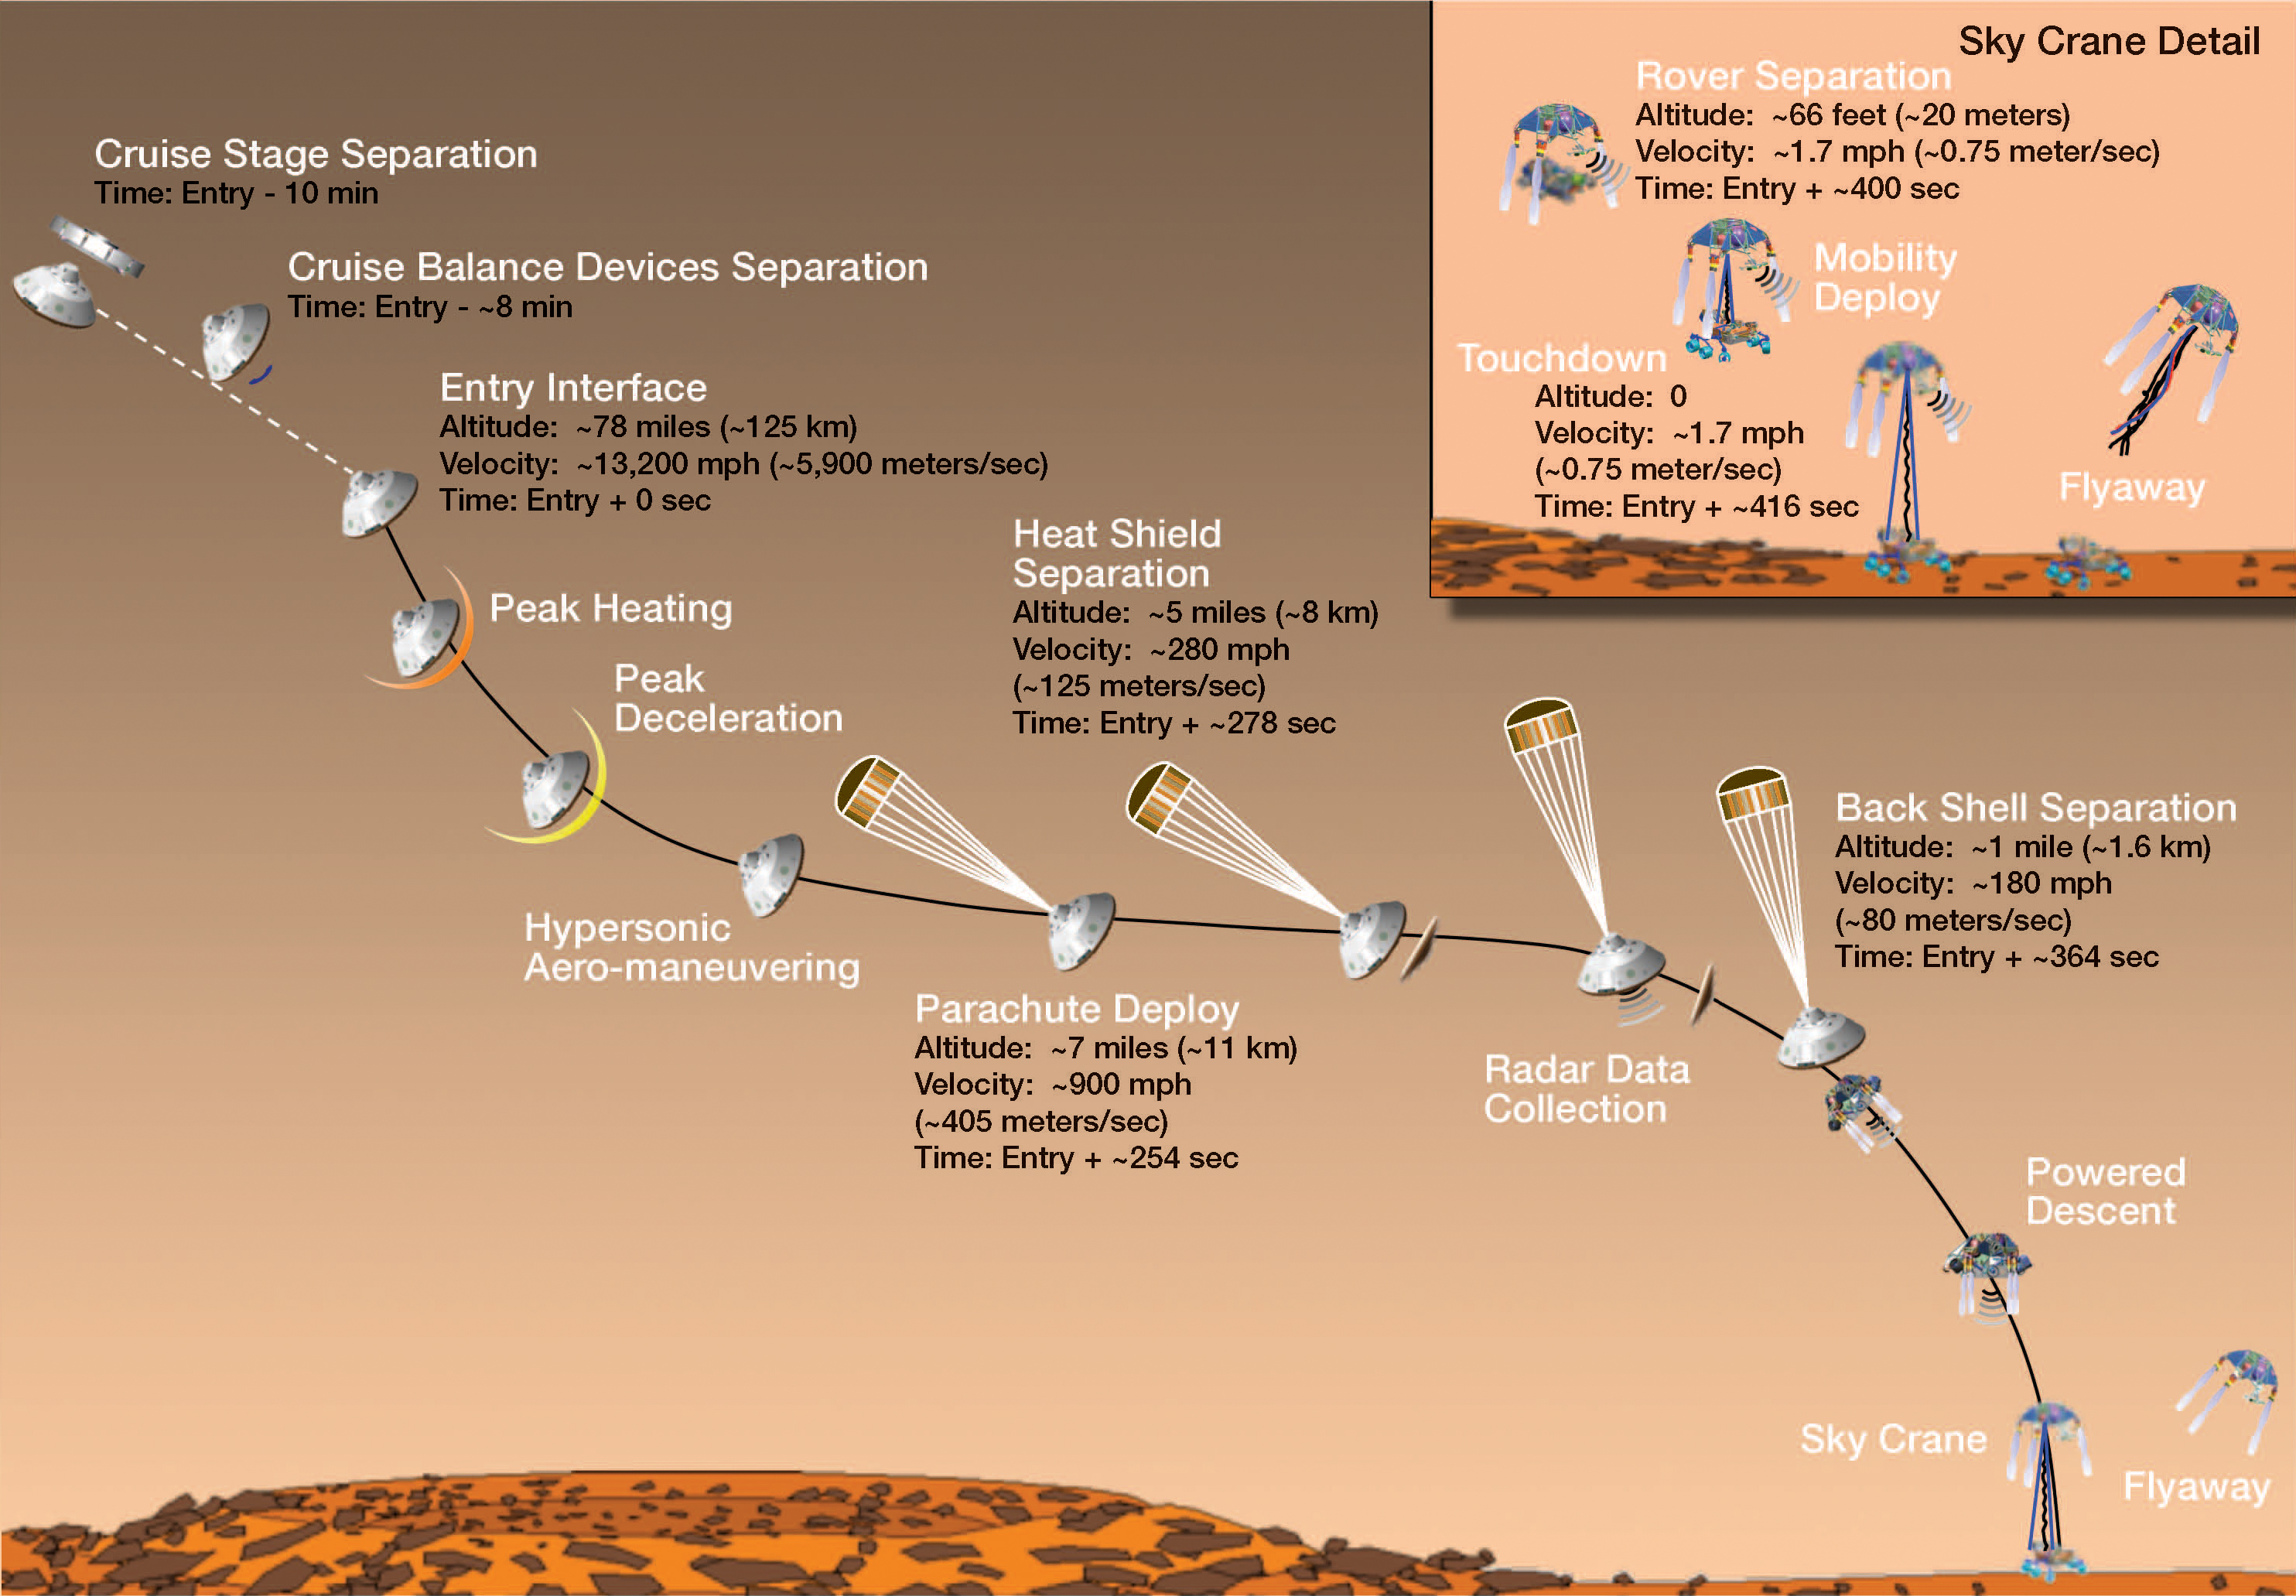
\includegraphics[width=0.45\textwidth]{Curiosity_landing.jpg}
\end{center}


\subsection*{Guided entry}
\initial{10} minutes before reaching the atmosphere the cruising stage is detached and burns up.
With a velocity of $21,240km/h$ it slams into the Martian atmosphere at an altitude of $125km$ \cite{NASALanding_diag}.
Creating so much aerodynamic drag the heat shield reach a temperature of $2100\degree C$ glowing white hot \cite{NASALanding} \cite{NASA_youtube}.
Being the first spacecraft to use precision landing techniques on Mars the name 'guided entry' refers to its ability to adjust it course during this first stage.
The course adjustments will be controlled by four sets of two Reaction Control System (RCS) thrusters.
Each pair capable of generation about $500N$ ($50kg$) of thrust \cite{HistoricLanding}.
Where the Mars Exploration Rovers could have landed anywhere within their respective $150$ by $20km$ landing ellipses, Curiosity landed within a $20km$ ellipse \cite{NASALanding}.
The Martian atmosphere is extremely difficult to slow down in because it has just enough atmosphere that you have to deal with it (or else your spacecraft is destroyed), but still too little to get the job done \cite{NASA_youtube}.
The heat shield only manages to slow the spacecraft to a speed of $1,620km/h$ in which time the deceleration has created a maximum force equal to $15G$s \cite{NASALanding} \cite{HistoricLanding}.
This is still way too fast for a safe landing and brings us to the next step.

\subsection*{Parachute descent}
\initial{A}t an altitude of $11km$, the largest and strongest supersonic parachute ever constructed for an extraterrestrial flight deploys \cite{NASALanding} \cite{Parachute}.
Deploying at such speeds creates a neck snapping $9G$s \cite{NASA_youtube}.
The parachute with a diameter of nearly $16m$ has 80 suspension lines measuring more than $50m$ in length and would be capable of generating $24,500kg$ of drag force \cite{Parachute}.
About $8km$ over the surface the heat shield poops of giving a clear view for the radar.
The radar calculates altitude and speed determining when to initiate the next phase \cite{NASALanding}.

The parachute will not be able to slow the spacecraft to a speed lower than about $280km/h$.
This is still way too fast for a landing. Only one solution; separate the rover from the backshell and parachute \cite{NASALanding}.

\subsection*{Powered descent}
\initial{T}he descent stage (includes the rover) now in free fall fires eight Aerojet's 'variable' thrust mono propellant hydrazine rocket thrusters and doing a divert maneuver to avoid colliding with the backshell and parachute \cite{NASALanding} \cite{HistoricLanding}.
Each of these rocket thrusters (called Mars Lander Engines or MLEs) are capable of producing $320kg$ of lift \cite{HistoricLanding}.
The MLEs will slow the spacecraft to a velocity of $14.5km/h$ while adjusting its position for the final stage. 

\subsection*{Sky crane}
\initial{A}t an altitude of $27m$, the rover is detached from the descent stage and slowly lowered to the ground.
While three nylon cords (communications between the rover and the descent stage is ensured by an umbilical line) lower the rover, the descent speed is reduced to $2.7km/h$.
At $7.5m$, the cords are fully extended and the descent speed is kept constant at $2.7km/h$ until the rover finally touches down \cite{NASALanding} \cite{HistoricLanding}.
The descent stages continues its descent velocity while the rover use $2s$ to confirm full weight on all wheels.
The cords and umbilical line pyrotechnically detaches from Curiosity and the descent stages assume command of itself.
Tilting $45\degree$, it performs a flyaway-maneuver crash-landing at least $150m$ away \cite{HistoricLanding}. 
Despite everything that could have gone wrong the rover landed unharmed on the surface of Mars at 10:32 p.m. PDT on Aug. 5 2012 \cite{NASALanding}.